\chapter{Progettazione Fisica e Alimentazione del Data Warehouse}

\section{Progettazione Fisica}
La progettazione logica di una base di dati definisce uno schema indipendente da come le informazioni vengono effettivamente memorizzate sul disco, garantendo così l'indipendenza logica. La progettazione fisica, al contrario, ha l'obiettivo di definire le strutture fisiche di memorizzazione e di accesso ai dati al fine di ottimizzare i tempi di esecuzione delle interrogazioni. 
Poiché SQL è un linguaggio dichiarativo (si specifica \textit{cosa} cercare e non \textit{come}), spetta a un modulo interno del DBMS, chiamato \textbf{ottimizzatore}, decidere il piano di esecuzione più efficiente. Il compito del progettista fisico è quindi fornire all'ottimizzatore le strutture accessorie adeguate.

\subsection{Caratteristiche del carico di lavoro nel Data Warehouse}
I sistemi di Data Warehouse sono progettati per soddisfare specifiche esigenze di analisi. Il carico di lavoro tipico presenta le seguenti caratteristiche:
\begin{itemize}
    \item \textbf{Interrogazioni complesse con aggregazioni:} Le query richiedono l'accesso a una frazione significativa di ogni tabella e comportano operazioni onerose come join tra tabelle di grandi dimensioni (la tabella dei fatti e le dimensioni) e raggruppamenti (\texttt{GROUP BY}).
    \item \textbf{Accesso in sola lettura:} Durante le normali operazioni di analisi, i dati non vengono modificati dagli utenti.
    \item \textbf{Aggiornamento periodico:} I dati vengono aggiornati in finestre temporali ben definite (es. ogni notte), momento in cui è necessario ricostruire o aggiornare anche le strutture fisiche di accesso, come gli indici e le viste.
\end{itemize}

\subsection{Viste Materializzate}
\subsubsection{Definizione e Differenza con le Viste Logiche}
Per abbattere i tempi di esecuzione delle operazioni più onerose (in particolare Join e \texttt{GROUP BY}), si utilizzano le \textbf{viste materializzate}.
A differenza delle \textit{viste logiche} studiate nelle basi di dati relazionali (che contengono solo la definizione della query, utile spesso per motivi di riservatezza, e vengono ricalcolate a ogni esecuzione), le viste materializzate sono \textbf{sommari precalcolati della tabella dei fatti, memorizzati esplicitamente sul disco}.

L'utente finale o l'analista non ha bisogno di conoscere l'esistenza di queste viste. Le interrogazioni vengono scritte facendo riferimento allo schema multidimensionale standard (tabella dei fatti e dimensioni). Sarà l'ottimizzatore del DBMS che, qualora riconosca che una vista materializzata precalcolata può rispondere in modo più efficiente alla query o a parte di essa, effettuerà in modo trasparente la riscrittura dell'interrogazione (meccanismo di \textit{aggregate navigation}).

\subsubsection{Creazione di una Vista Materializzata}
Una vista materializzata si definisce tramite un'istruzione SQL. Al suo interno contiene tipicamente:
\begin{itemize}
    \item Un'operazione di Join tra la tabella dei fatti e le dimensioni di interesse.
    \item Una clausola \texttt{GROUP BY} per precalcolare l'aggregazione, riducendo il dettaglio delle dimensioni originali.
    \item Funzioni di aggregazione (come \texttt{SUM}, \texttt{COUNT}, ecc.) sulle misure.
\end{itemize}

% FIGURA ORIGINALE DA RECUPERARE DALLE SLIDE
% Slide di provenienza: Viste materializzate (Definizione di v3)
% Tipo: Tabella/Codice SQL
% Descrizione: Esempio di definizione della vista materializzata v3
% Punto di inserimento: Qui, per mostrare la sintassi SQL della vista
% File da inserire: def_vista_v3
\begin{figure}[H]
    \centering
    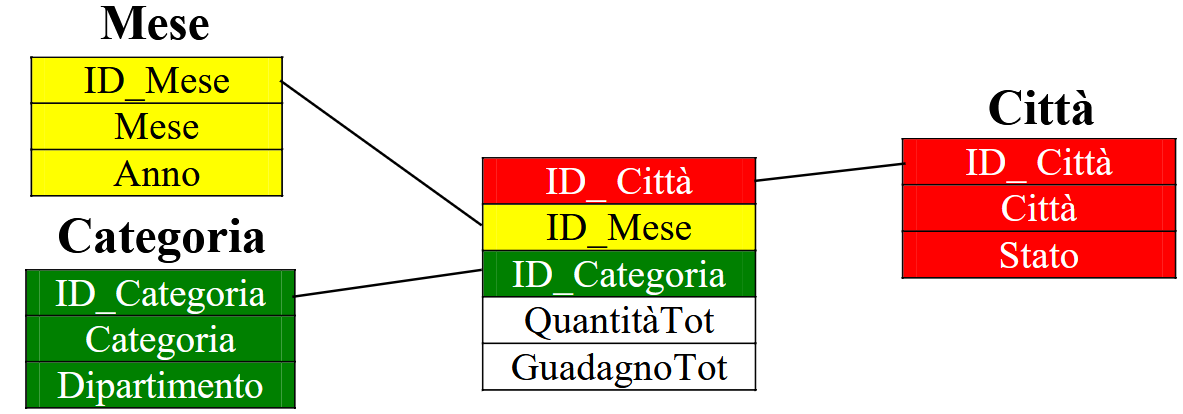
\includegraphics[width=0.7\textwidth]{capitoli/05_Data warehouse_progettazione fisica e alimentazione/images/def_vista_v3}
    \caption{Definizione SQL di una vista materializzata.}
    \label{fig:def-vista-v3}
\end{figure}

\noindent\textbf{Avvertenza sulle metriche:} Una singola vista materializzata può essere utilizzata per rispondere a più interrogazioni diverse, aggregando ulteriormente i dati precalcolati. Tuttavia, bisogna prestare estrema attenzione all'operatore di aggregazione. Ad esempio, non è possibile calcolare la media delle medie. Le metriche memorizzate nella vista devono permettere il calcolo corretto ai livelli di dettaglio superiori (ad esempio, memorizzando somma e conteggio anziché direttamente la media).

\subsubsection{Il Reticolo Multidimensionale}
Per visualizzare le possibili aggregazioni e le dipendenze tra di esse, si utilizza il \textbf{reticolo multidimensionale} (o reticolo delle viste). Ogni nodo del reticolo rappresenta una possibile granularità (una combinazione di attributi dimensionali). 

Il nodo di partenza (spesso in basso) rappresenta il dettaglio massimo presente nella tabella dei fatti (es. Prodotto, Data, Negozio). Risalendo le gerarchie delle dimensioni, si ottengono viste via via più aggregate (es. Categoria, Mese, Città).
Se esiste un collegamento diretto (un arco) tra un nodo $A$ e un nodo $B$ posizionato più in alto, significa che il risultato della vista $A$ può essere utilizzato per calcolare il risultato della vista $B$. 

% FIGURA ORIGINALE DA RECUPERARE DALLE SLIDE
% Slide di provenienza: Reticolo multidimensionale
% Tipo: Grafo/Schema concettuale
% Descrizione: Reticolo che mostra i nodi delle viste (V2, V3, V4, ecc.) e i collegamenti tra le aggregazioni possibili.
% Punto di inserimento: Qui, per illustrare le dipendenze tra i livelli di raggruppamento.
% File da inserire: reticolo_viste
\begin{figure}[H]
    \centering
    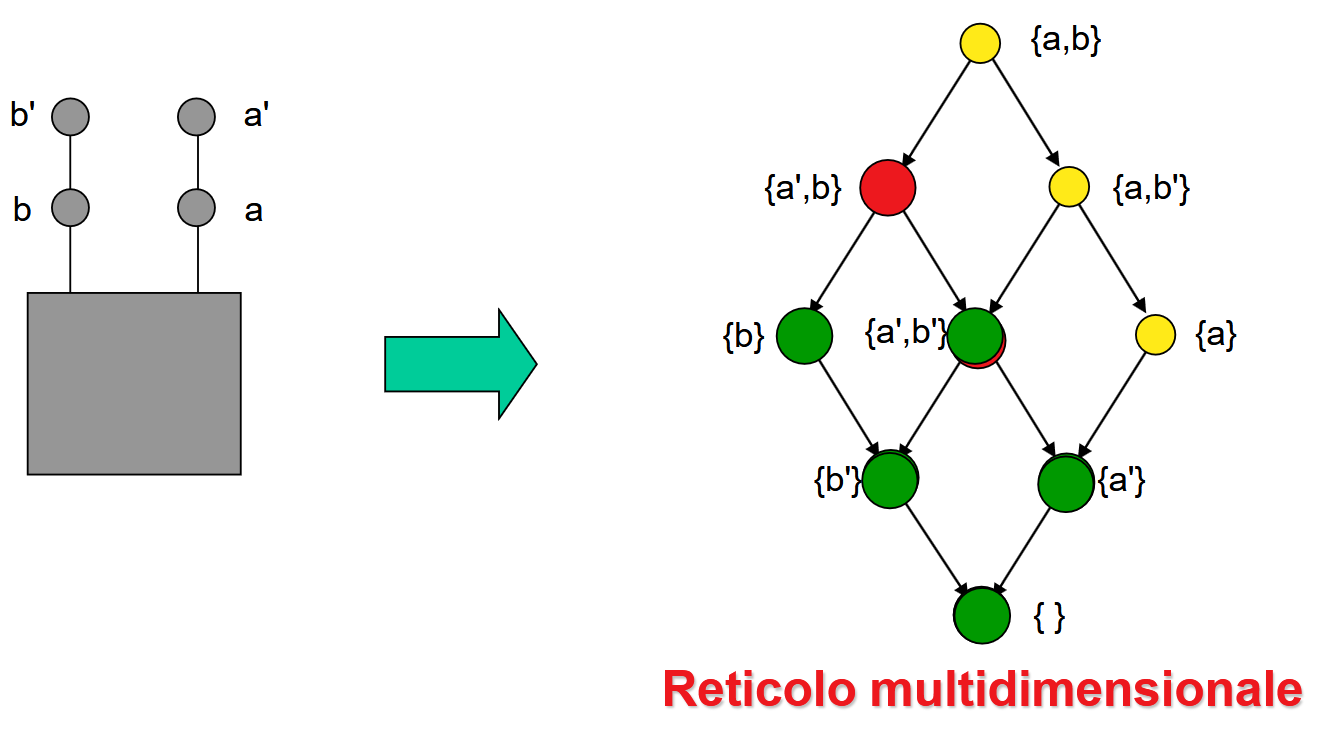
\includegraphics[width=0.85\textwidth]{capitoli/05_Data warehouse_progettazione fisica e alimentazione/images/reticolo_viste}
    \caption{Esempio di reticolo multidimensionale che illustra le dipendenze tra le viste materializzabili.}
    \label{fig:reticolo-viste}
\end{figure}

\noindent\textbf{L'importanza delle Gerarchie:}
Durante la lezione, il professore ha sottolineato un errore concettuale comune nella lettura del reticolo. Affinché si possa aggregare da un livello a un altro (es. da Tipo Prodotto a Categoria, o da Città a Regione), deve esistere un vincolo gerarchico rigoroso. 
Ad esempio, dati come Data, Mese e Trimestre formano una gerarchia rigida. Al contrario, se Tipo e Categoria fossero dimensioni ortogonali (dove a un tipo non è associata una sola categoria univoca, come giorno della settimana e mese), non ci potrebbe essere un arco diretto nel reticolo. Il reticolo assume quindi validità solo se supportato dalla corretta definizione delle gerarchie dimensionali.

\subsubsection{Il Problema della Scelta delle Viste}
Il numero di possibili viste materializzabili in un Data Warehouse reale è enorme. Non è pensabile materializzarle tutte. La scelta costituisce un problema di ottimizzazione che mira a minimizzare specifiche funzioni di costo:
\begin{itemize}
    \item Il costo di esecuzione delle interrogazioni (che si abbassa aumentando le viste).
    \item Il costo di aggiornamento delle viste stesse (che si alza aumentando le viste, poiché a ogni refresh del data warehouse le viste vanno ricalcolate).
\end{itemize}
A ciò si aggiungono dei vincoli pratici:
\begin{itemize}
    \item Spazio su disco disponibile.
    \item Finestra temporale disponibile per l'aggiornamento notturno (se l'aggiornamento richiede 8 ore ma la finestra utile è di sole 4 ore, il sistema non è sostenibile).
\end{itemize}

% FIGURA ORIGINALE DA RECUPERARE DALLE SLIDE
% Slide di provenienza: Scelta delle viste (Sequenza di 4 slide)
% Tipo: Diagramma a barre/Grafico intuitivo
% Descrizione: Istogrammi che confrontano il tempo di esecuzione, il tempo di aggiornamento e lo spazio occupato tra tre soluzioni: una singola vista generale, tre viste specifiche, o una soluzione intermedia.
% Punto di inserimento: Qui, a supporto della spiegazione dei trade-off.
% File da inserire: grafici_scelta_viste
\begin{figure}[H]
    \centering
    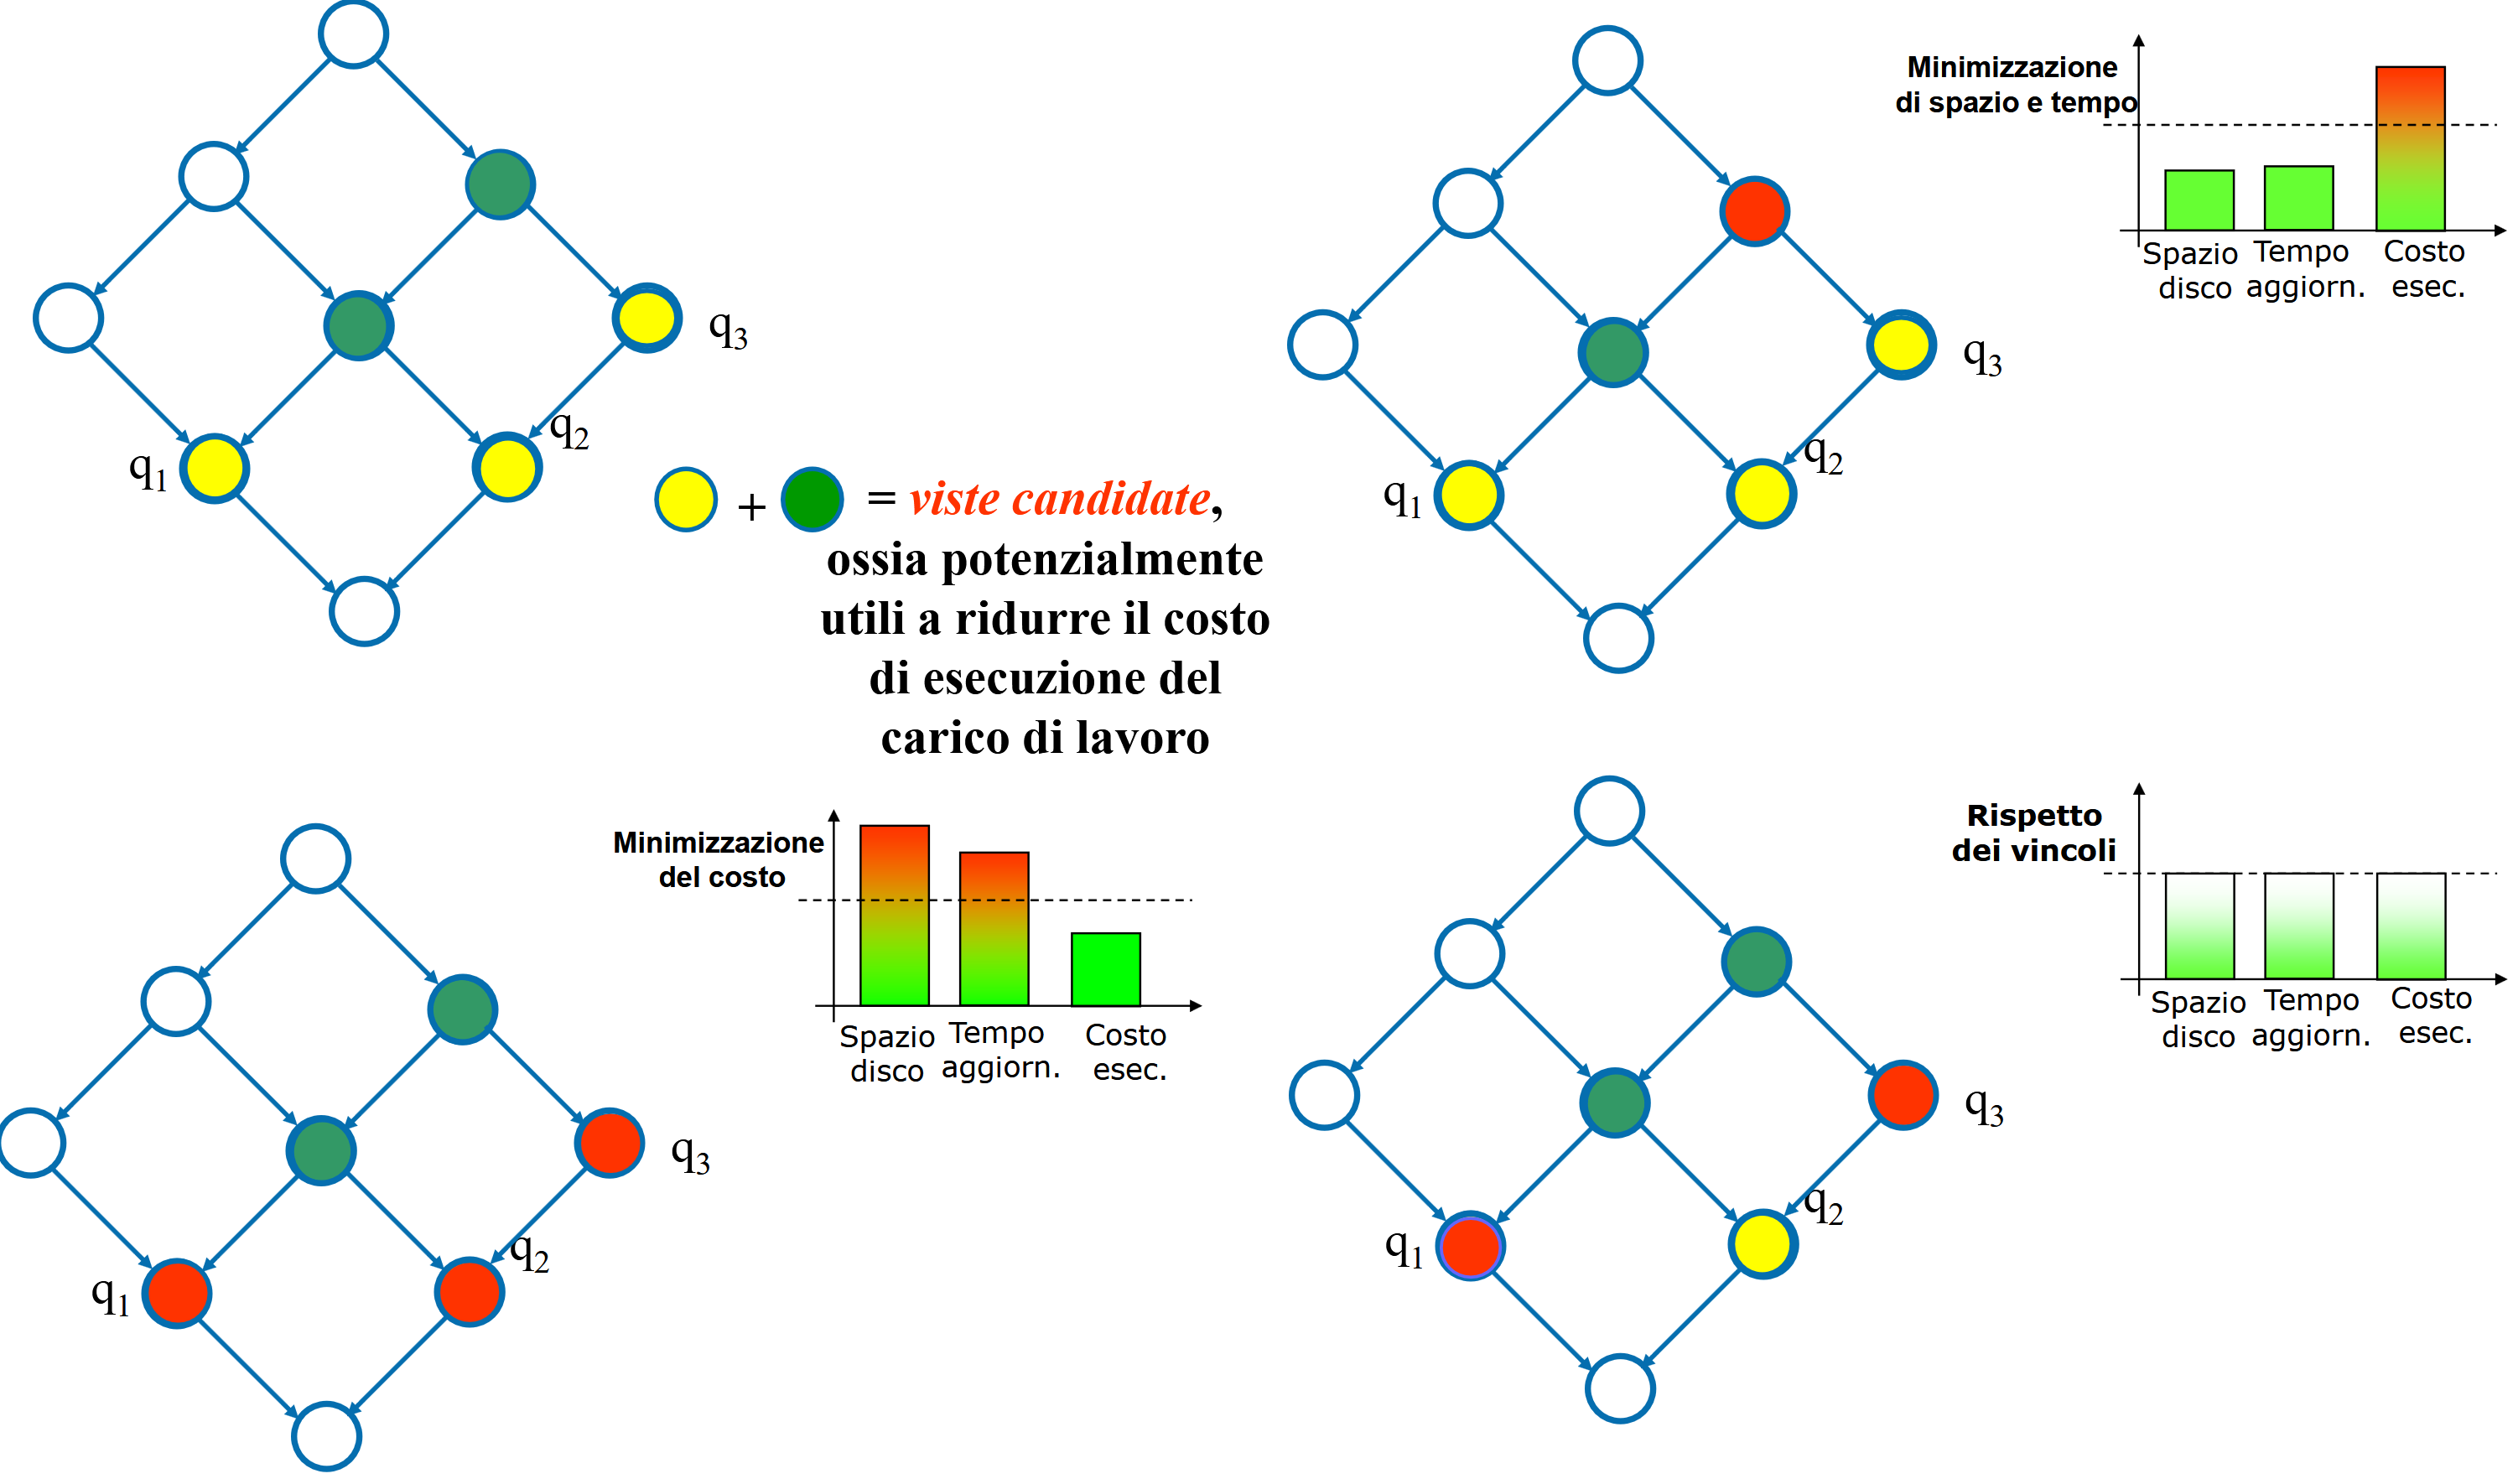
\includegraphics[width=0.9\textwidth]{capitoli/05_Data warehouse_progettazione fisica e alimentazione/images/grafici_scelta_viste}
    \caption{Analisi dei costi per la scelta delle viste ottimali: bilanciamento tra spazio, tempo di aggiornamento e tempo di query.}
    \label{fig:scelta-viste-costi}
\end{figure}

In sintesi, si può optare per tre strategie principali (illustrate nell'esempio discusso in aula per risolvere tre specifiche query):
\begin{enumerate}
    \item \textbf{Una sola vista aggregata molto specifica (basso livello):} Risponde a tutte le interrogazioni. Occupa più spazio e ha un tempo di esecuzione medio-alto per query molto aggregate, ma è l'unica vista da mantenere aggiornata.
    \item \textbf{Viste separate e mirate per ogni query:} Tempi di esecuzione minimi, ma massima occupazione di spazio e massimo costo di manutenzione/aggiornamento.
    \item \textbf{Soluzione intermedia:} Creare alcune viste intermedie nel reticolo che riescano a servire più query contemporaneamente offrendo il miglior compromesso tra tempo di risposta e costi di manutenzione.
\end{enumerate}

\subsection{Altre Strutture Fisiche: Indici e Parallelismo}
Oltre alle viste materializzate, la progettazione fisica si avvale di altre strutture:
\begin{itemize}
    \item \textbf{Indici B+-tree:} Poco adatti per gli attributi dimensionali del data warehouse che spesso hanno una cardinalità bassa (es. sesso, stato civile, regione).
    \item \textbf{Indici Bitmap e Indici di Join:} Strutture più efficienti per gli attributi dimensionali, frequentemente coinvolti nei predicati di selezione e nelle operazioni di join.
\end{itemize}
Il \textbf{tuning} del database è la fase operativa in cui, tramite il monitoraggio, si verifica se l'ottimizzatore sta effettivamente utilizzando gli indici e le viste creati dal progettista. In caso contrario, queste strutture fisiche consumano risorse (per l'aggiornamento) senza portare alcun beneficio e vanno rimosse o modificate.
Inoltre, le interrogazioni complesse (specialmente Join e Group By) beneficiano enormemente del \textbf{parallelismo} (frammentazione dei dati, e parallelizzazione inter-query e intra-query).

\section{Alimentazione del Data Warehouse (Processo ETL)}
L'architettura del Data Warehouse prevede che i dati di analisi siano fisicamente separati da quelli dei sistemi operazionali (sorgenti). Per mantenere aggiornato il Data Warehouse, è necessario un processo denominato \textbf{ETL} (Extraction, Transformation and Loading).
Spesso, tra le sorgenti e il data warehouse, si inserisce un'area di appoggio intermedia detta \textbf{Staging Area}, che porta l'architettura a tre livelli e facilita l'esecuzione di trasformazioni complesse.

Il processo ETL deve gestire due scenari ben distinti:
\begin{enumerate}
    \item \textbf{Il primo popolamento (tempo zero):} Il Data Warehouse e le dimensioni sono completamente vuoti e occorre acquisire una fotografia storica completa di tutto il periodo di interesse aziendale.
    \item \textbf{L'aggiornamento periodico (es. giornaliero):} Il Data Warehouse è già popolato, bisogna estrarre e caricare unicamente le variazioni e le nuove transazioni avvenute dall'ultimo caricamento.
\end{enumerate}

\subsection{Estrazione (Extraction)}
L'estrazione è la fase di acquisizione dei dati dalle sorgenti. Può essere:
\begin{itemize}
    \item \textbf{Statica:} Una vera e propria fotografia dell'intero database operazionale, eseguita per il primo popolamento.
    \item \textbf{Incrementale:} Si estraggono solo i dati inseriti, modificati o cancellati dall'ultimo aggiornamento.
\end{itemize}

\subsubsection{Le sfide dell'Estrazione Incrementale}
La complessità dell'estrazione incrementale dipende fortemente dalla natura dei dati operazionali:
\begin{itemize}
    \item \textbf{Dati storicizzati:} Il sistema OLTP salva storicamente tutte le variazioni (es. transazioni bancarie). L'estrazione è semplice perché ogni evento è tracciato.
    \item \textbf{Dati semi-storicizzati o Transitori:} Il DBMS mantiene solo l'immagine corrente del dato (es. scorte di magazzino in un dato istante) sovrascrivendo i valori precedenti. L'estrazione incrementale è molto complessa perché si perde traccia di cosa sia cambiato e di eventuali cancellazioni.
\end{itemize}

Per comprendere questa complessità, consideriamo il seguente esempio di estrazione incrementale tra il 4 aprile e il 6 aprile.

\begin{table}[H]
    \centering
    \caption{Fotografia DBMS al 4/4/2010}
    \begin{tabular}{cllc}
    \toprule
    \textbf{CodProdotto} & \textbf{Cliente} & \textbf{Qtà} \\
    \midrule
    1 & Greco di tufo & Malavasi & 50 \\
    2 & Barolo & Maio & 150 \\
    3 & Barbera & Lumini & 75 \\
    4 & Sangiovese & Cappelli & 45 \\
    \bottomrule
    \end{tabular}
\end{table}

\begin{table}[H]
    \centering
    \caption{Fotografia DBMS al 6/4/2010}
    \begin{tabular}{cllc}
    \toprule
    \textbf{Cod} & \textbf{Prodotto} & \textbf{Cliente} & \textbf{Qtà} \\
    \midrule
    1 & Greco di tufo & Malavasi & 50 \\
    2 & Barolo & Maio & 150 \\
    4 & Sangiovese & Cappelli & 145 \\
    5 & Vermentino & Maltoni & 25 \\
    6 & Trebbiano & Maltoni & 150 \\
    \bottomrule
    \end{tabular}
\end{table}

Un sistema ETL efficiente deve dedurre dalla differenza tra questi stati un file di aggiornamento che tracci esattamente le operazioni logiche avvenute, non potendosi limitare alle sole letture:

\begin{table}[H]
    \centering
    \caption{Estrazione Incrementale risultante (D=Delete, U=Update, I=Insert)}
    \begin{tabular}{cllcl}
    \toprule
    \textbf{Cod} & \textbf{Prodotto} & \textbf{Cliente} & \textbf{Qtà} & \textbf{Azione} \\
    \midrule
    3 & Barbera & Lumini & 75 & D (cancellato) \\
    4 & Sangiovese & Cappelli & 145 & U (modifica qtà da 45 a 145)\\
    5 & Vermentino & Maltoni & 25 & I (nuovo inserimento)\\
    6 & Trebbiano & Maltoni & 150 & I (nuovo inserimento)\\
    \bottomrule
    \end{tabular}
\end{table}

\subsubsection{Tecniche per l'estrazione incrementale}
Per realizzare concretamente questa estrazione, si possono utilizzare diverse tecniche, ognuna con precisi trade-off:

\begin{table}[H]
    \centering
    \resizebox{\textwidth}{!}{%
    \begin{tabular}{lccccc}
    \toprule
    & \textbf{Statica} & \textbf{Marche temp.} & \textbf{Assistita appl.} & \textbf{Trigger} & \textbf{Log} \\
    \midrule
    Gestione dati transitori & NO & Incompleta & Completa & Completa & Completa \\
    Supporto sistemi a file & SI & SI & SI & SI & NO \\
    Complessità procedure & Bassa & Bassa & Alta & Media & Bassa \\
    Modifiche ad applicazioni& Nessuna & Probabile & Probabile & Nessuna & Nessuna \\
    Impatto prestazioni operaz.& Nessuna & Nessuna & Medio & Medio & Nessuna \\
    \bottomrule
    \end{tabular}%
    }
    \caption{Confronto semplificato tra le tecniche di estrazione (rielaborato dalle slide).}
    \label{tab:tecniche-estrazione}
\end{table}

\begin{itemize}
    \item \textbf{Assistita dall'applicazione:} L'applicativo stesso viene modificato per scrivere da qualche parte i dati che sta cambiando. Richiede modifiche ai programmi (applicazioni on top al DBMS) e aumenta il carico applicativo, ma è spesso l'unica via per i vecchi sistemi \textit{legacy}.
    \item \textbf{Uso del Log:} Si legge il file di log interno del DBMS (che per sua natura traccia ogni operazione per garantire la recovery). È molto efficiente e non impatta sul carico applicativo, ma il log è in formato proprietario del vendor del database.
    \item \textbf{Tramite Trigger:} Si programmano dei trigger interni al DBMS che scattano autonomamente su \texttt{INSERT}, \texttt{UPDATE} e \texttt{DELETE}. Non richiede la modifica del programma applicativo esterno, ma incrementa notevolmente il carico di lavoro del DBMS in fase transazionale.
    \item \textbf{Tramite Timestamp (Marche temporali):} Si aggiunge una colonna data/ora ai record per tracciare l'ultima modifica. È un metodo parziale perché fallisce nel tracciare i dati \textit{cancellati} (se il record scompare, scompare anche il suo timestamp).
\end{itemize}

\subsection{Pulitura (Data Cleansing)}
I dati estratti da sorgenti eterogenee presentano quasi sempre problemi di \textit{Data Quality}: duplicati, dati mancanti, formati non uniformi (es. "C.so" vs "Corso"), valori errati.
Le procedure di pulitura includono:
\begin{itemize}
    \item \textbf{Uso di dizionari:} Standardizzazione dei domini (es. unificare le sigle delle province, CAP validi).
    \item \textbf{Tecniche di fusione approssimata (Approximate Join e Purge/Merge):} Spesso uno stesso cliente è memorizzato in due filiali con grafie leggermente diverse (es. "Rossi M." e "Mario Rossi"). Non avendo una chiave univoca comune, bisogna applicare algoritmi di similarità testuale per identificare se si tratta della stessa entità e procedere all'unione dei record (purge/merge).
\end{itemize}

\noindent\textbf{Nota sull'Intelligenza Artificiale nell'ETL:}
Come sottolineato dal professore durante la lezione, i sistemi ETL moderni si stanno evolvendo rapidamente. Per affrontare problemi di pulitura complessa (come join approssimati senza chiavi certe o riconoscimento di entità), si sta diffondendo l'uso di tecniche di Data Science, inclusi algoritmi di clustering e l'uso di modelli linguistici di grandi dimensioni (LLM). L'ETL non è più solo una semplice procedura SQL, ma assomiglia sempre di più alla fase di \textit{data preparation} del Machine Learning.

% FIGURA ORIGINALE DA RECUPERARE DALLE SLIDE
% Slide di provenienza: Join approssimato / Purge/Merge / Esempio di pulitura
% Tipo: Esempi visivi e schemi
% Descrizione: Esempio di standardizzazione anagrafica (es. "Elena Baralis C.so Duca...") e schema del join approssimato.
% Punto di inserimento: Qui, a corredo della spiegazione del cleansing.
% File da inserire: schemi_pulitura
\begin{figure}[H]
    \centering
    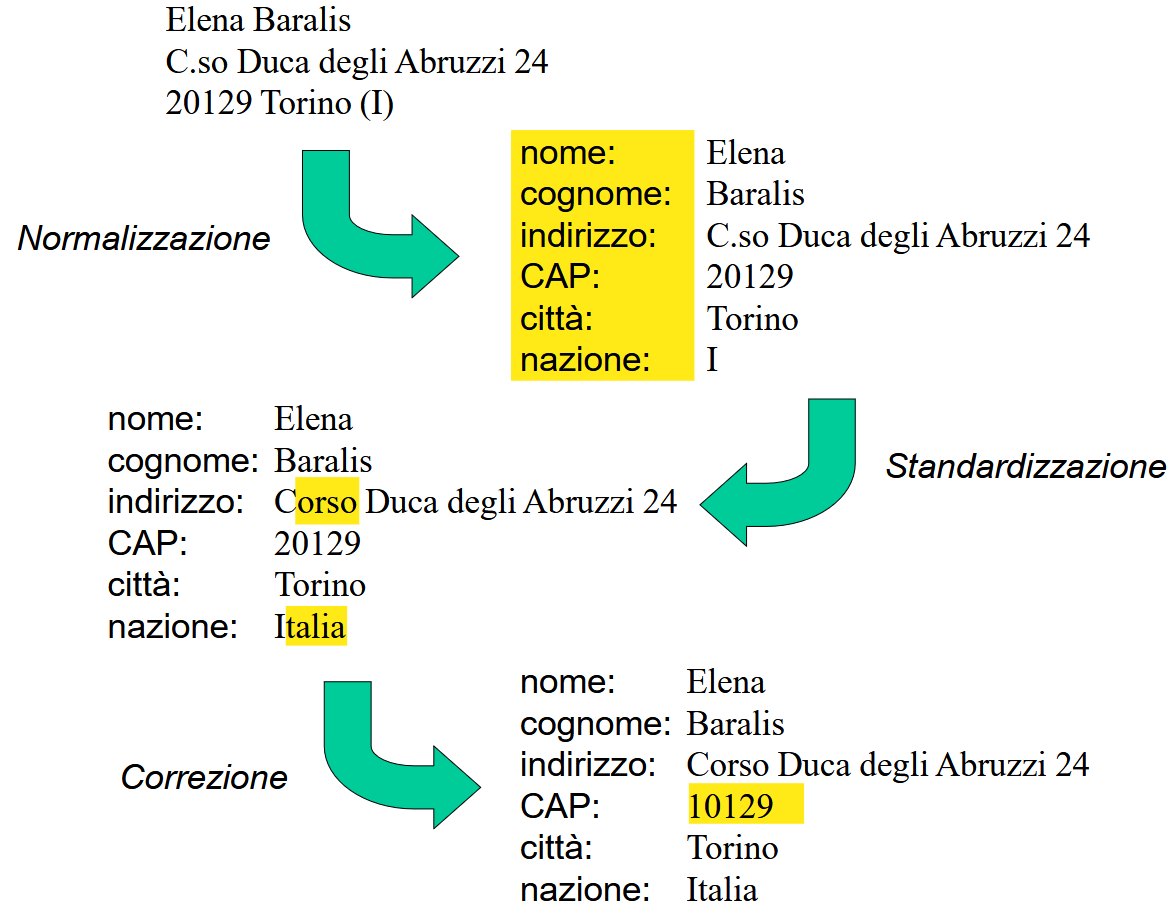
\includegraphics[width=0.75\textwidth]{capitoli/05_Data warehouse_progettazione fisica e alimentazione/images/schemi_pulitura}
    \caption{Esempi operativi di pulitura e risoluzione del problema del Purge/Merge.}
    \label{fig:schemi-pulitura}
\end{figure}

\subsection{Trasformazione}
Questa fase converte i dati dal formato in cui sono memorizzati operazionalmente a quello integrato del data warehouse. Questo passaggio, che di norma si completa nella Staging Area, prevede:
\begin{itemize}
    \item Passaggio allo \textbf{schema riconciliato} (notazione uniforme).
    \item Generazione dei \textbf{valori aggregati} se richiesti dallo schema.
    \item \textbf{Generazione delle chiavi surrogate:} Fondamentale per svincolare l'identificativo interno del data warehouse dalle chiavi applicative (che potrebbero cambiare nel tempo nei sistemi sorgente o presentare conflitti).
\end{itemize}

\subsection{Caricamento (Loading)}
La fase finale è la propagazione dei dati trasformati fisicamente nel Data Warehouse. 
Esiste una \textbf{gerarchia rigorosa e obbligatoria} per l'ordine di caricamento, al fine di rispettare l'integrità referenziale. I passi sono i seguenti:
\begin{enumerate}
    \item \textbf{Alimentazione delle Dimensioni:} Prima di poter caricare un evento, le entità che lo descrivono devono esistere. 
    Il sistema legge gli aggiornamenti dalla Staging Area, verifica se il record dimensionale esiste già (es. un cliente). Se esiste, ne estrae la \textit{chiave surrogata}; se non esiste, inserisce il nuovo record generando una nuova chiave.
    \item \textbf{Alimentazione della Fact Table:} I nuovi eventi vengono inseriti nella tabella dei fatti. Durante questo inserimento, il sistema non usa i codici operazionali originali, ma recupera (tramite query) le \textit{chiavi surrogate} che sono state appena aggiornate/generate nel passo 1.
    \item \textbf{Aggiornamento delle Viste Materializzate e degli Indici:} Poiché i dati di base sono cambiati, tutte le strutture fisiche di supporto (che contengono aggregazioni precalcolate) devono essere riallineate con i nuovi valori.
\end{enumerate}

% FIGURA ORIGINALE DA RECUPERARE DALLE SLIDE
% Slide di provenienza: Alimentazione delle dimensioni / Alimentazione delle fact table
% Tipo: Diagramma di flusso
% Descrizione: Diagrammi di flusso che mostrano la logica di inserimento dei dati nelle dimensioni (verifica esistenza -> insert/select) e l'inserimento nella fact table tramite lookup delle chiavi surrogate.
% Punto di inserimento: Qui, a chiusura del capitolo sull'ETL per mostrare visivamente la logica di caricamento.
% File da inserire: diagrammi_caricamento
\begin{figure}[H]
    \centering
    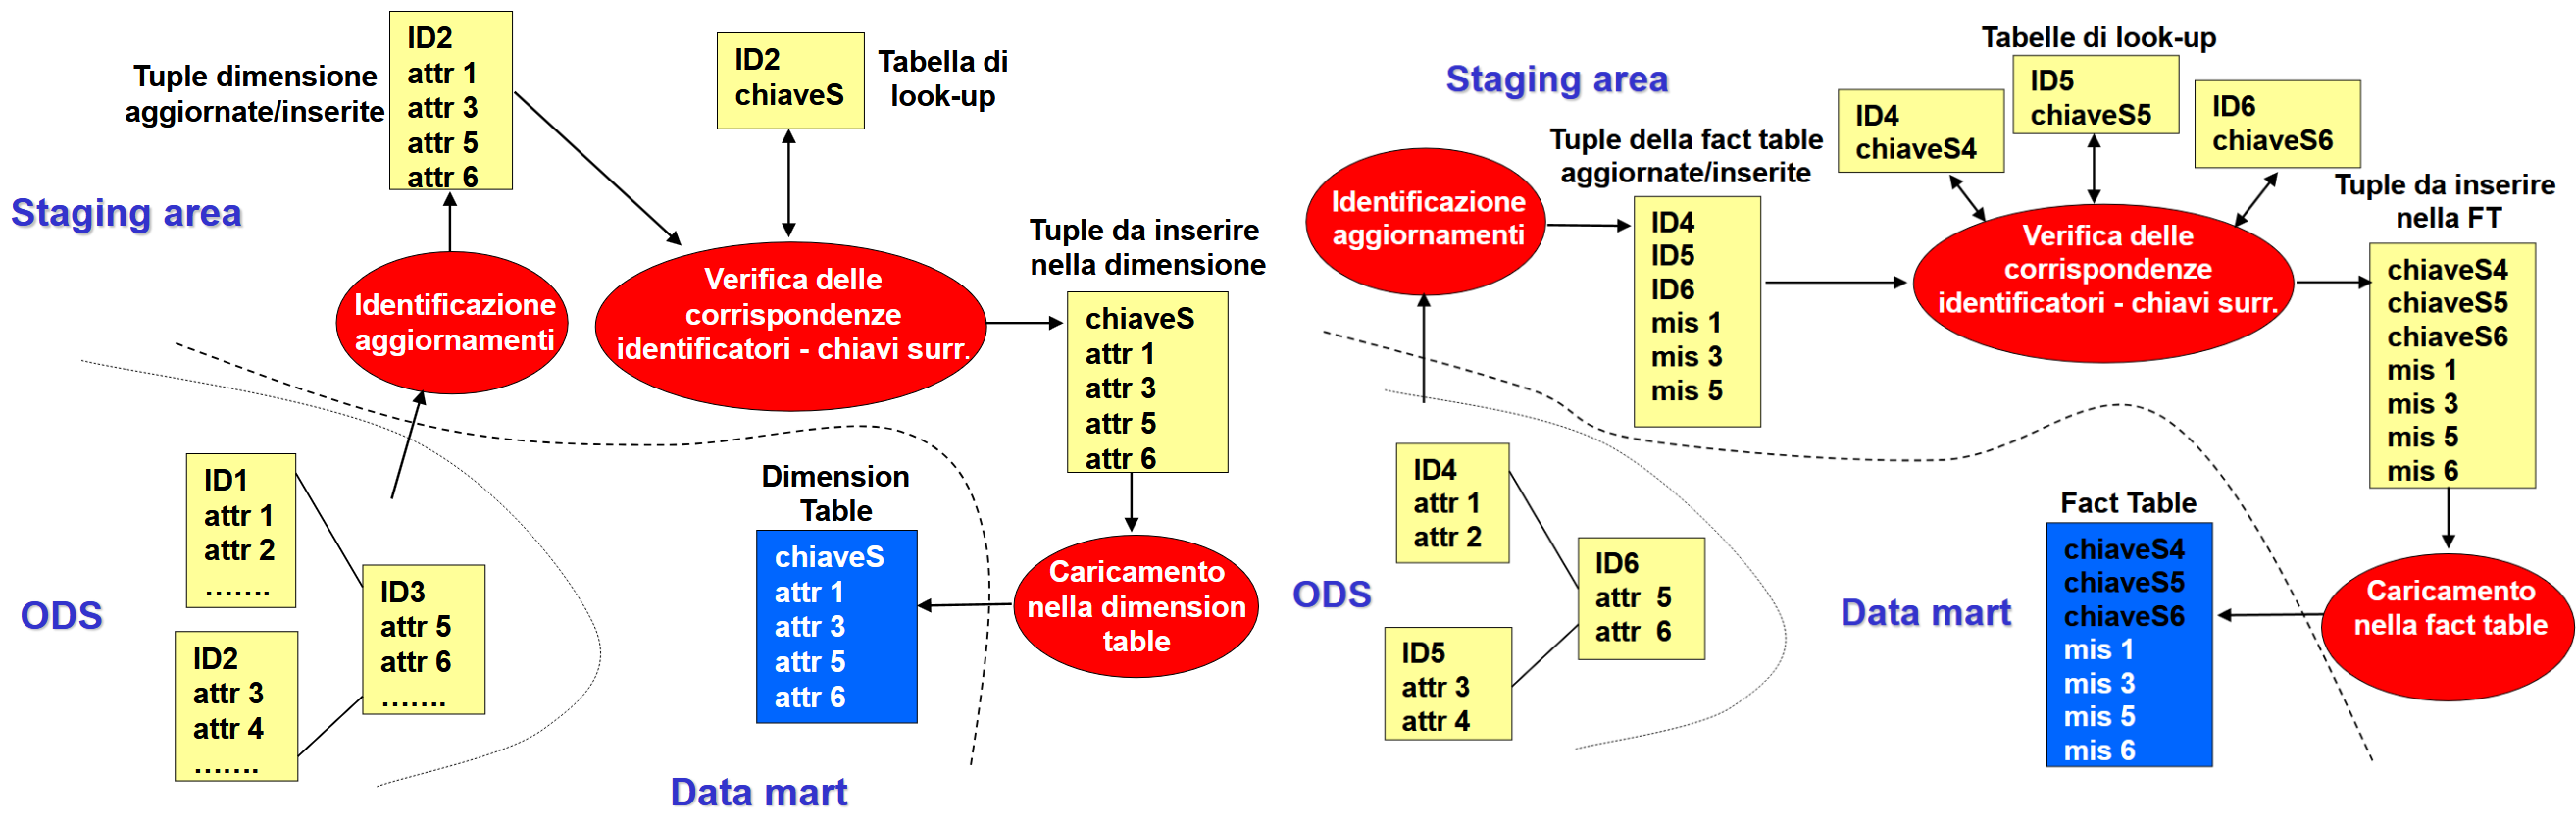
\includegraphics[width=1\textwidth]{capitoli/05_Data warehouse_progettazione fisica e alimentazione/images/diagrammi_caricamento}
    \caption{Flusso logico per l'alimentazione delle dimensioni e della fact table.}
    \label{fig:diagrammi-caricamento}
\end{figure}